\chapter{Theory}

This work showcases the use of \glspl{pomdp} to model and solve decision making
problems in robotics with inherent uncertainty. In order to provide a baseline
for further discussions of specific application domains
(\cref{chap:applications}) we first introduce some of the throughout this work.
It should be noted that in the interest of conciseness we focus this
theoretical introduction on only the main tools use. Fundamental concepts of
statistical inference and tools like \textit{Monte Carlo Integration} are
assumed to be known. For a thorough discussion of these underlying concept the
reader may refer to \cite{kochenderfer2015decision} as well as
\cite{probRobotics}.\todo{Can I also assume knowledge of fully observable
MDPs?}

In the following, we first introduce the theoretical framework of \glspl{pomdp}
(\cref{sec:pomdp}). This section discusses modelling assumptions, structure
of solutions as well as theoretical properties of \glspl{pomdp}. Thereafter,
\cref{sec:online-pomdp-solvers} describes two state-of-the-art online solution
methods for problems of this domain.

\section{Partially Observable Markov Decision Processes}\label{sec:pomdp}

A \acf{pomdp} is a principled mathematical formalism capable of representing
a broad range of sequential decision making problems under uncertainty. As the
name suggests, this framework is a generalization of the more popular \ac{mdp}
to the partially observable case. The graphical representation of a \ac{pomdp}
as dynamic decision network is depicted in \cref{fig:pomdp}.

\begin{figure}[htpb]
  \centering
  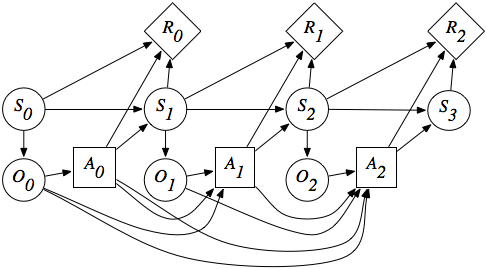
\includegraphics[width=.7\textwidth]{pomdp-dynamic-decision-network.png}
  \caption{The POMDP as a dynamic decision network. \todo[inline]{Replace with
  vector graphics.}}
  \label{fig:name}
\end{figure}

\todo[inline]{brief definition of solutions to POMDPs as "conditional plans"
and point out that in general the full solution is intractable. Point to
complexity theory with some good source for this. (e.g. Mykel)}

\todo[inline]{Theoretical properties by modelling things in such a way. What
can be gained? What is the difference?}

\section{Online POMDP Solvers}\label{sec:online-pomdp-solvers}

\todo[inline]{The solvers described here were chosen as they are state of the
art and show good perfomance over a range of problems. Point to Zach's paper
for solver perfomance comparison and DESPOT paper.}

\section{POMCPOW}

\todo[inline]{write:}
\begin{itemize}
  \item explain the basic idea of POMCPOW as Monte Carlo with DPW.
  \item is extension of POMCP with weighted particle beliefs.
\end{itemize}
\missingfigure{Pseudo Code with formal description in text.}

\missingfigure{graphical model of POMCP-Tree with weighted scenarios.}

\section{DESPOT}

\todo[inline]{write:}
\begin{itemize}
  \item formal, high-level idea of a DESPOT (idea of scenarios etc.)
  \item the search algorithm on a DESPOT with bounds
  \item explain the difference to POMCPOW (or Monte Carlo methods in general)
  \item point to literature for convergence guarantees
\end{itemize}

\missingfigure{DESPOT tree visualization}
\missingfigure{DESPOT algorithm Pseudo Code}

